\documentclass[11pt]{article}

\usepackage[a4paper,margin=24mm]{geometry}
\usepackage{amsmath,amssymb,mathtools}
\usepackage{booktabs,longtable,array}
\usepackage{enumitem}
\usepackage{xcolor}
\usepackage{hyperref}
\usepackage{graphicx,pdflscape}
\usepackage{fontspec}
\usepackage{fvextra}
\usepackage{etoolbox,needspace}

\setmainfont{Times New Roman}
\setsansfont{Arial}
\setmonofont{Consolas}
\hypersetup{
  colorlinks=true,
  linkcolor=blue!55!black,
  urlcolor=blue!55!black,
  pdftitle={Formalization Architecture and Lean Infrastructure for the Rate--Distortion Theorem}
}
\setlist{nosep,leftmargin=1.6em}
\setlength{\parindent}{1.5em}
\setlength{\parskip}{0.15em}
\emergencystretch=3em

\definecolor{codebg}{HTML}{F5F7F9}
\definecolor{ruleblue}{HTML}{315B7D}
\definecolor{softgray}{HTML}{F0F2F4}
\DefineVerbatimEnvironment{LeanCode}{Verbatim}{
  fontsize=\small,
  breaklines=true,
  breakanywhere=true,
  frame=single,
  rulecolor=\color{ruleblue},
  fillcolor=\color{codebg},
  framesep=3mm
}

\newcommand{\PMF}{\operatorname{PMF}}
\BeforeBeginEnvironment{LeanCode}{\par\noindent\begin{minipage}{\linewidth}}
\AfterEndEnvironment{LeanCode}{\end{minipage}\par\medskip}
\newcommand{\E}{\mathbb{E}}
\newcommand{\Var}{\operatorname{Var}}
\newcommand{\RD}{R_I}
\newcommand{\MI}{I}
\newcommand{\KL}{D_{\mathrm{KL}}}
\newcommand{\dmax}{d_{\max}}
\newcommand{\Nbar}{\overline{\mathbb{N}}}

\title{Formalization Architecture and Lean Infrastructure\\
for the Finite-Alphabet Rate--Distortion Theorem}
\author{Fubin Yan}
\date{Updated reference, 22 September 2026}

\begin{document}
\raggedbottom
\maketitle

\begin{abstract}
This document describes the Lean 4 formalization of the finite-alphabet
rate--distortion theorem in \path{RateDistortion.lean}.
The development is organized as reusable information-theoretic infrastructure,
not as a single proof script for the final theorem.  It builds finite-PMF
expectation and variance, Shannon and conditional entropy, a bridge from
mathlib's measure-theoretic Kullback--Leibler divergence to finite entropy
formulas, memoryless block sources and channels, information density, weak-law
bounds, random-codebook covering, deterministic codebook extraction,
single-letterization for arbitrary deterministic codes, asymptotic code
sequences, and a diagonal argument that removes the positive coding slacks.

The final public API proves strict achievability with every code satisfying
the prescribed rate bound, and the converse at every distortion threshold.
It also proves equality-rate achievability when $\RD(P,d,D)$ is finite under
an asymptotic rate constraint. Compactness of the finite test-channel space,
continuity, and lower semicontinuity establish right continuity within the
development. This report describes the reusable infrastructure and distinguishes
the two operational rate constraints.
\end{abstract}

\tableofcontents

\section{Purpose and contribution}

The classical rate--distortion theorem relates two descriptions of lossy source
coding.  The information quantity is
\[
  \RD(P,d,D)
  = \inf_{W:\,\E_{P W}[d(X,Y)]\le D} \MI_{P W}(X;Y),
\]
where $P$ is a source distribution and $W(y\mid x)$ is a test channel.  The
operational quantity is obtained from sequences of finite-block deterministic
encoders and decoders whose asymptotic rate and expected distortion are bounded.

The formalization has two goals:
\begin{enumerate}
  \item verify the direct and converse proof chains for finite alphabets;
  \item provide stable finite-information-theory APIs that later developments
        can reuse for channel coding, source coding, typicality, concentration,
        and other single-letterization arguments.
\end{enumerate}

Lean forces several conventions to be explicit.  Blocklength zero cannot be
silently divided away; distortion values and possibly infinite thresholds must
live in compatible ordered types; the KL and entropy definitions must be shown
to agree; attainment of the infimum defining $\RD$ requires a proof; a fixed-slack code
for every sufficiently large blocklength is not yet a single sequence with
vanishing slack; and an asymptotic converse at $D+\varepsilon$ does not imply a
converse at $D$ without a continuity argument.  These issues determine the
architecture of the Lean code.

\section{Architecture at a glance}

Figure~\ref{fig:lean-dependency} is a declaration-level dependency graph
extracted from the compiled Lean environment.  It is not a manually asserted
outline: every arrow is backed by a path of constant references in declaration
types, definition bodies, or theorem proofs. Hidden helper declarations are traversed
until another selected public declaration is reached, and the resulting graph
is transitively reduced.  Thus an arrow $A\to C$ is omitted when the displayed
graph already contains a path $A\to\cdots\to C$.

\begin{landscape}
\begin{figure}[p]
  \centering
  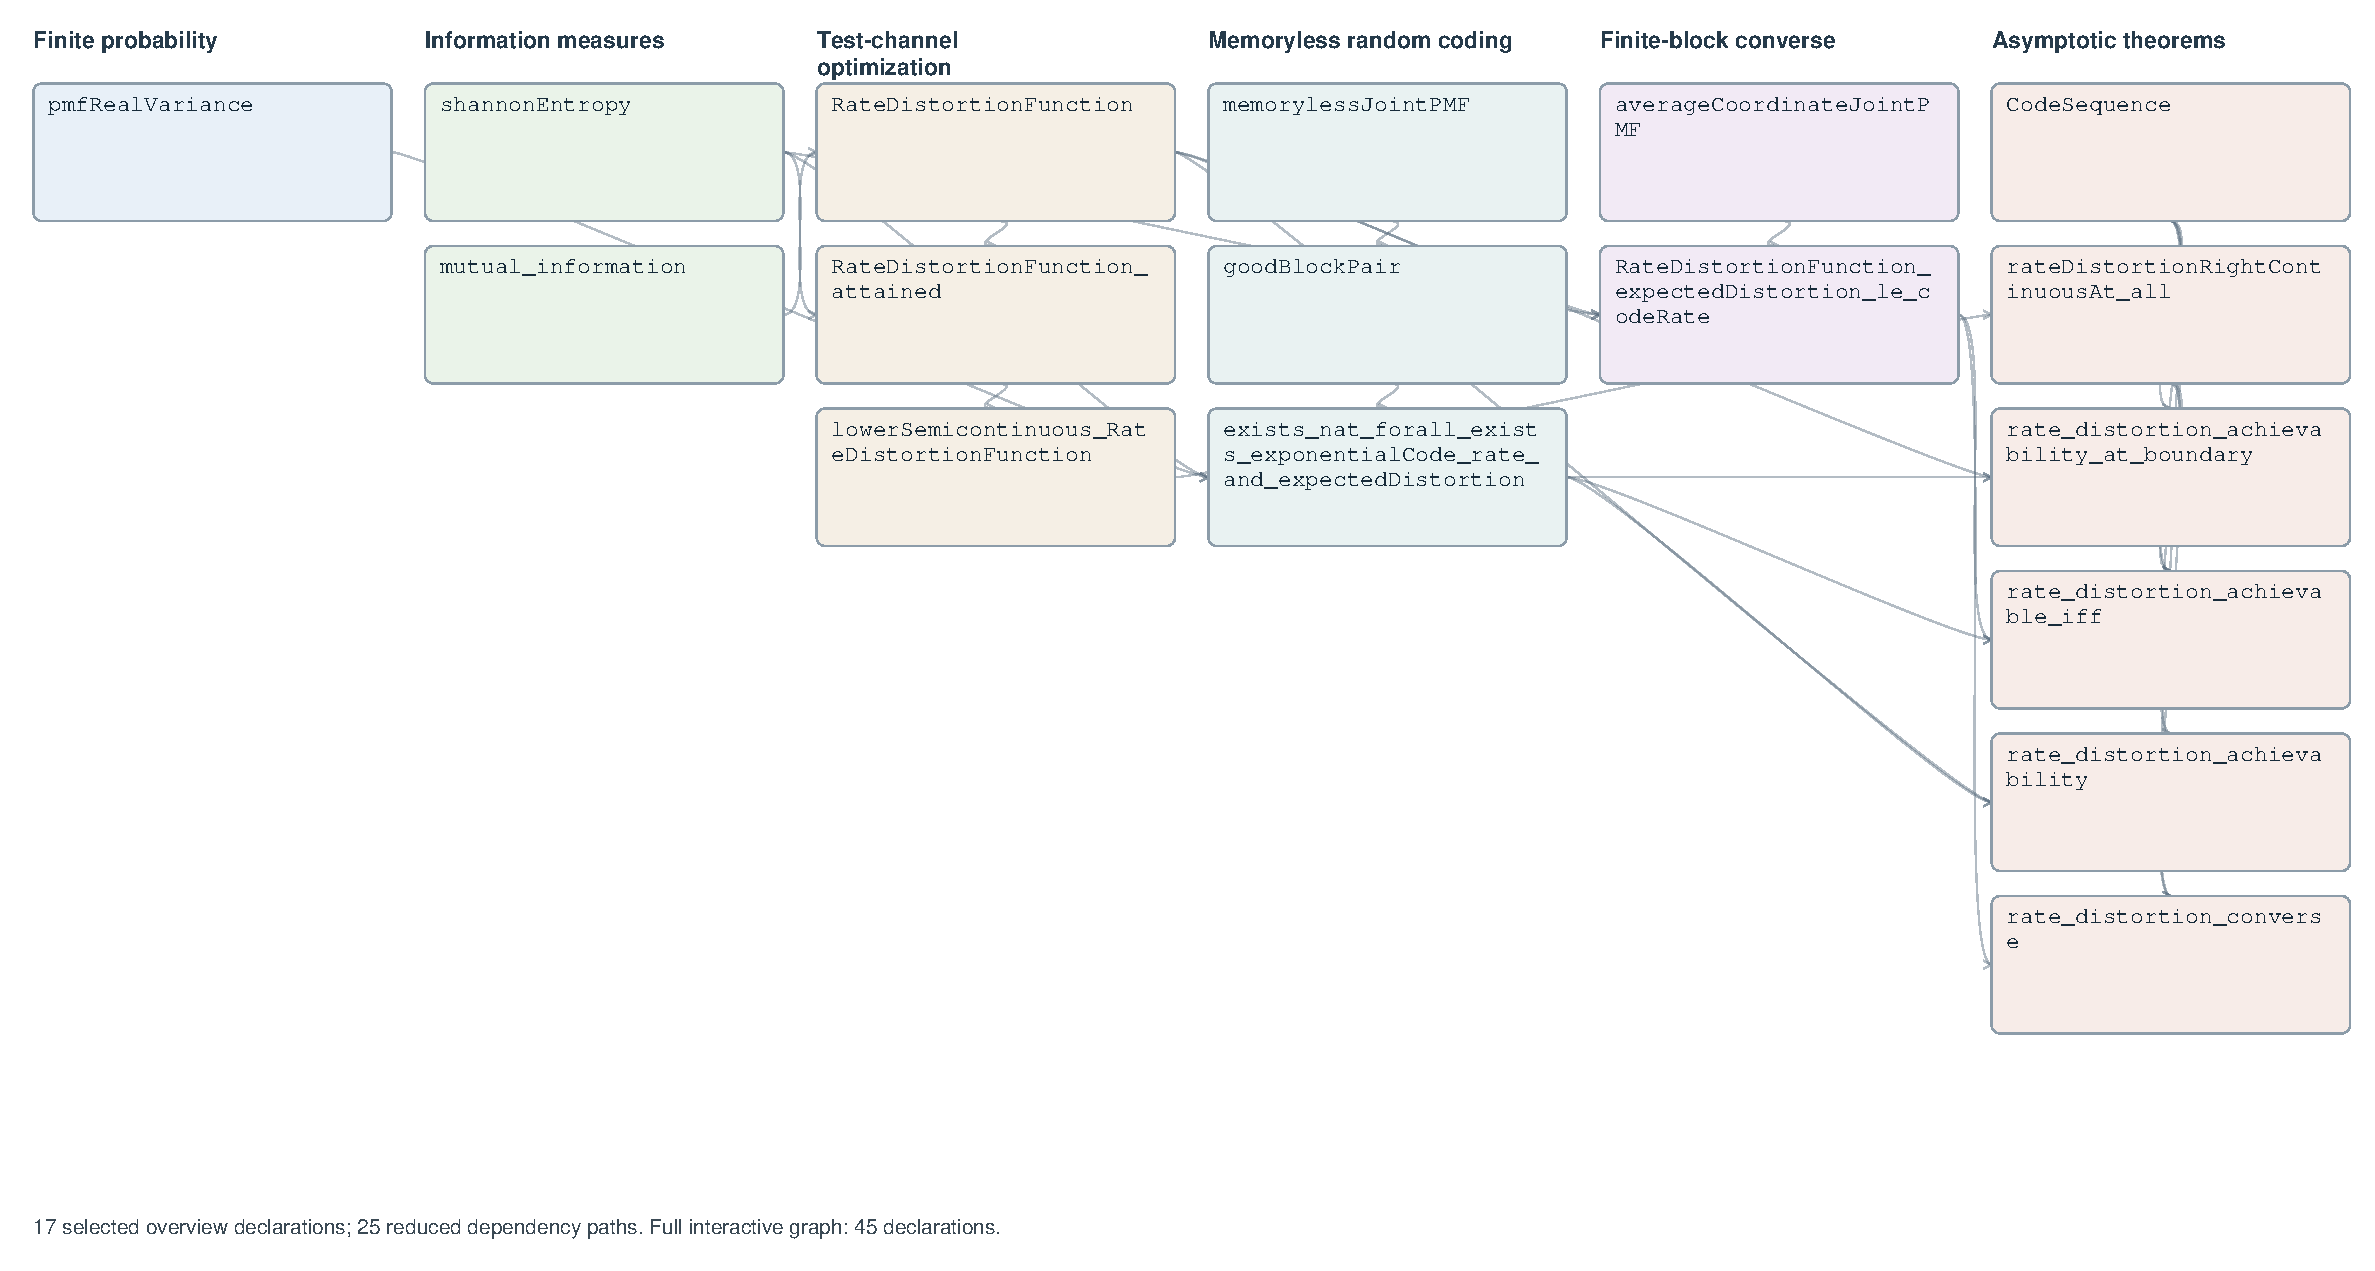
\includegraphics[width=0.94\linewidth]{rate_distortion_dependency_graph_report.pdf}
  \caption{Machine-extracted Lean dependency overview. Arrows point from prerequisites to declarations that use them, preserving dependency paths through hidden declarations. The interactive graph retains the full selected-declaration view and distinguishes references in statement types from references in proof terms and definition bodies.}
  \label{fig:lean-dependency}
\end{figure}
\end{landscape}

The reproducible extraction script is
\path{GenerateDependencyGraph.lean}.  It uses Lean's
\texttt{Constant\allowbreak Info.get\allowbreak Used\allowbreak Constants\allowbreak As\allowbreak Set} API on the compiled module.  The
machine-readable output is
\path{rate_distortion_dependencies.json};
\path{GenerateDependencyArtifacts.ps1} merges duplicate statement/proof edges
and computes the transitive reduction.  The stand-alone file
\path{rate_distortion_dependency_graph.html} provides search, core/full views,
edge-type filtering, and clickable upstream/downstream inspection without an
external web service.

There are two distinct proof-oriented endpoints.  The direct part constructs
codes from a test channel and then diagonalizes shrinking error tolerances.  The
converse part turns an arbitrary block code into a single-letter joint law and
then passes its finite-block inequality to a limsup. Both connect the
single-letter function \texttt{Rate\allowbreak Distortion\allowbreak Function} with the operational
definitions \texttt{is\allowbreak Achievable\allowbreak Pointwise} and \texttt{is\allowbreak Achievable}.

The current implementation is a single source file.  Its internal layering is
mathematically coherent, but the dependency graph suggests a future split into
modules for finite PMFs, entropy, memoryless blocks, random coding, converse,
and asymptotics.  Section~\ref{sec:extensions} records that extension path.

\section{Formal setting and representation choices}

\subsection{Finite alphabets}

The entire development works with finite source and reproduction alphabets:

\begin{LeanCode}
variable {X Y : Type*}
  [Fintype X] [Fintype Y] [DecidableEq X] [DecidableEq Y]
\end{LeanCode}

The use of \texttt{Fintype} makes probabilities, expectations, entropy, and
event probabilities finite sums.  This permits an elementary random-coding
formalization while still using mathlib's canonical \texttt{PMF} type.
Theorems such as \texttt{nonempty\_\allowbreak of\_\allowbreak pmf} and
\texttt{nonempty\_\allowbreak reproduction\_\allowbreak of\_\allowbreak source\_\allowbreak channel} recover nonemptiness from
actual probability data instead of adding global \texttt{Nonempty} assumptions.

\subsection{Distortion and boundedness}

The single-letter distortion is finite and nonnegative:
\[
  d:X\times Y\longrightarrow \mathbb{R}_{\ge 0}.
\]

\begin{LeanCode}
def Distortion := X -> Y -> NNReal

noncomputable def distortionBound
    (d : Distortion (X := X) (Y := Y)) : NNReal :=
  Finset.univ.sup (fun x => Finset.univ.sup (fun y => d x y))

theorem distortion_le_bound
    (d : Distortion (X := X) (Y := Y)) (x : X) (y : Y) :
    d x y <= distortionBound d
\end{LeanCode}

Choosing \texttt{NNReal} rather than \texttt{ENNReal} for each value of $d$
rules out an infinite letterwise distortion.  Because both alphabets are finite,
the global bound $\dmax$ is then derived rather than assumed.  Expected
distortions and distortion thresholds use \texttt{ENNReal}; hence limits,
infima, and the value $\top$ remain available at the analytic layer.

This division of roles is important:
\[
  d(x,y)\in\mathbb{R}_{\ge0},\qquad
  \E[d]\in[0,\infty],\qquad D\in[0,\infty].
\]
The code proves that all expectations generated by finite distortion remain
below the finite coercion of $\dmax$.

\subsection{Blocks and positive blocklengths}

Blocks are functions on \texttt{Fin n}:

\begin{LeanCode}
abbrev Xblock (n : Nat) (X : Type*) := Fin n -> X
abbrev Yblock (n : Nat) (Y : Type*) := Fin n -> Y
abbrev Index (M : Nat) := Fin M
\end{LeanCode}

For $n>0$, block distortion and code rate are
\[
  d_n(x^n,y^n)=\frac1n\sum_{i\in\mathrm{Fin}(n)}d(x_i,y_i),
  \qquad r(n,M)=\frac{\log M}{n}.
\]

\begin{LeanCode}
def blockDistortion (hn : 0 < n)
    (d : Distortion (X := X) (Y := Y))
    (x : Xblock n X) (y : Yblock n Y) : ENNReal :=
  (∑ i : Fin n, (d (x i) (y i) : ENNReal)) / n

def codeRate (hn : 0 < n) : Real := Real.log M / n
\end{LeanCode}

The proof witness \texttt{hn : 0 < n} is part of both definitions.  At the
sequence level the actual blocklength at index $k$ is $k+1$, so zero-length
codes never enter the operational theorem.

\section{Finite-PMF probability infrastructure}

The formalization introduces a small real-valued expectation and variance API
for finite PMFs:
\[
  \E_P[f]=\sum_a P(a)f(a),\qquad
  \Var_P(f)=\sum_a P(a)(f(a)-\E_P[f])^2.
\]

\begin{LeanCode}
noncomputable def pmfRealExpectation
    (P : PMF A) (f : A -> Real) : Real :=
  ∑ a : A, (P a).toReal * f a

noncomputable def pmfRealVariance
    (P : PMF A) (f : A -> Real) : Real :=
  ∑ a : A, (P a).toReal *
    (f a - pmfRealExpectation P f) ^ 2
\end{LeanCode}

The corresponding reusable API includes:
\begin{itemize}
  \item normalization in \texttt{ENNReal} and after \texttt{to\allowbreak Real};
  \item expectation under \texttt{PMF.map};
  \item linearity for addition and scalar multiplication;
  \item invariance of variance under a PMF map;
  \item product-distribution expectation and variance formulas;
  \item a finite-sum Chebyshev inequality,
  \[
    P\{|f-\E f|\ge\varepsilon\}
      \le \frac{\Var(f)}{\varepsilon^2}.
  \]
\end{itemize}

The Chebyshev theorem is stated directly as a finite PMF sum.  This is a
deliberate boundary: no measurable-space structure is needed for elementary
finite concentration, while the KL layer below still reuses mathlib's
measure-theoretic information theory.

Other broadly reusable finite-PMF lemmas include change of variables for
\path{map}, a law-of-total-expectation identity for \path{bind}, support
transport, and the probabilistic-method lemma
\path{exists_le_pmf_weighted_sum}, which extracts an outcome whose value
is no greater than its PMF-weighted average.

\section{Entropy, KL divergence, and mutual information}

\subsection{Shannon and conditional entropy}

Entropy is real-valued and measured in nats:
\[
  H(P)=-\sum_x P(x)\log P(x).
\]

\begin{LeanCode}
noncomputable def shannonEntropy (P : PMF X) : Real :=
  ∑ x : X, Real.negMulLog (P x).toReal

noncomputable def conditionalEntropy (Q : PMF (X × Y)) : Real :=
  shannonEntropy Q - shannonEntropy (Q.map Prod.fst)
\end{LeanCode}

The entropy infrastructure proves nonnegativity, the cardinality bound
$H(P)\le\log|X|$, entropy decrease under deterministic maps, invariance under
injective maps, the product formula, joint subadditivity, strong subadditivity,
and ``conditioning reduces entropy.''  The block converse later reuses the
coordinate form
\[
  H(Y^n\mid X^n)\le \sum_{i=1}^n H(Y_i\mid X_i).
\]

\subsection{KL-based and entropy-based mutual information}

The primary extended-nonnegative mutual information is built from mathlib's
KL divergence:
\[
  \MI_Q(X;Y)=\KL(Q\,\|\,Q_X\otimes Q_Y).
\]

\begin{LeanCode}
noncomputable def kl_divergence (P Q : PMF X) : ENNReal :=
  letI : MeasurableSpace X := top
  InformationTheory.klDiv P.toMeasure Q.toMeasure

def product_pmf (P_X : PMF X) (P_Y : PMF Y) : PMF (X × Y) :=
  P_X.bind (fun x => P_Y.map (fun y => (x, y)))

noncomputable def mutual_information (Q : PMF (X × Y)) : ENNReal :=
  kl_divergence Q (product_pmf (Q.map Prod.fst) (Q.map Prod.snd))
\end{LeanCode}

For algebraic finite proofs, the development also uses
\[
  I_H(Q)=H(Q_X)+H(Q_Y)-H(Q).
\]

\begin{LeanCode}
noncomputable def mutualInformationEntropy (Q : PMF (X × Y)) : Real :=
  shannonEntropy (Q.map Prod.fst) +
    shannonEntropy (Q.map Prod.snd) - shannonEntropy Q

theorem mutual_information_eq_ofReal_entropy (Q : PMF (X × Y)) :
  mutual_information Q =
    ENNReal.ofReal (mutualInformationEntropy Q)
\end{LeanCode}

This bridge is a central interface theorem.  Its proof establishes absolute
continuity of a finite joint PMF with respect to the product of its marginals,
identifies the Radon--Nikodym derivative with an explicit PMF density ratio,
and evaluates mathlib's log-likelihood integral as a finite entropy sum.
Consequently downstream proofs can use real arithmetic for entropy identities
and return to \texttt{ENNReal} at public boundaries.

The same layer defines conditional PMFs from arbitrary joint laws and proves
that every finite joint PMF is reconstructed as the joint induced by its first
marginal and conditional channel.  This is later used to formulate the
rate--distortion function both through channels and through arbitrary joint
laws with prescribed source marginal.

\section{The single-letter rate--distortion function}

For a source PMF $P$, distortion $d$, and threshold $D$, the information
rate--distortion function is the infimum over test channels:
\[
  \RD(P,d,D)=
  \inf\{\MI(P;W):\E_{PW}[d(X,Y)]\le D\}.
\]

\begin{LeanCode}
noncomputable def RateDistortionFunction
    (P : PMF X) (d : Distortion (X := X) (Y := Y))
    (D : ENNReal) : ENNReal :=
  sInf {r : ENNReal | exists W : X -> PMF Y, And
    (expected_distortion_single P W d <= D)
    (mutual_information (induced_joint P W) = r)}
\end{LeanCode}

The definition uses \texttt{s\allowbreak Inf} rather than assuming an optimizer.  This
choice supports the exact selection theorem needed by strict achievability:

\begin{LeanCode}
theorem exists_testChannel_of_RateDistortionFunction_lt_ofReal
    (hR : RateDistortionFunction P d D < ENNReal.ofReal R) :
  exists W : X -> PMF Y, And
    (expected_distortion_single P W d <= D)
    (mutualInformationEntropy (induced_joint P W) < R)
\end{LeanCode}

The main analytic API proves:
\begin{itemize}
  \item \texttt{Rate\allowbreak Distortion\allowbreak Function\_\allowbreak le}: every admissible test channel
        supplies an upper bound;
  \item \texttt{Rate\allowbreak Distortion\allowbreak Function\_\allowbreak antitone}: $D_1\le D_2$ implies
        $\RD(D_2)\le\RD(D_1)$;
  \item \texttt{Rate\allowbreak Distortion\allowbreak Function\_\allowbreak convex\_\allowbreak of\_\allowbreak feasible}: channel
        mixtures give convexity on feasible distortion levels;
  \item finiteness of $\RD(D)$ at feasible levels;
  \item $\RD(D)=0$ strictly above the zero-rate distortion threshold;
  \item attainment at feasible thresholds, lower semicontinuity, and right
        continuity at every distortion threshold.
\end{itemize}

The distortion-domain predicates are:
\begin{LeanCode}
def feasibleDistortion (P : PMF X) (d : Distortion) (D : ENNReal) : Prop :=
  exists W : X -> PMF Y, expected_distortion_single P W d <= D

noncomputable def minimumDistortion (P : PMF X) (d : Distortion) : ENNReal :=
  sInf (Set.range (fun W : X -> PMF Y =>
    expected_distortion_single P W d))

noncomputable def zeroRateDistortion (P : PMF X) (d : Distortion) : ENNReal :=
  sInf (Set.range (fun Q : PMF Y =>
    expected_distortion_single P (fun _ => Q) d))

def interiorDistortion (P : PMF X) (d : Distortion) (D : ENNReal) : Prop :=
  And (minimumDistortion P d < D) (D < zeroRateDistortion P d)
\end{LeanCode}

Right continuity is proved rather than postulated. The finite PMF space is
compact in the topology of pointwise convergence. Expected distortion and
mutual information are continuous on the test-channel space. Therefore a
nonempty feasible set admits an optimal channel in
\texttt{Rate\allowbreak Distortion\allowbreak Function\_\allowbreak attained}. Compactness also yields
\texttt{lower\allowbreak Semicontinuous\_\allowbreak Rate\allowbreak Distortion\allowbreak Function}; together with
monotonicity, this proves \texttt{rate\allowbreak Distortion\allowbreak Right\allowbreak Continuous\allowbreak At\_\allowbreak all}.
The older interior and strictly feasible specializations remain available,
but the final converse does not require their additional hypotheses.

\section{Memoryless block infrastructure}

The i.i.d. source and memoryless test channel are explicit finite PMFs:
\[
  P^n(x^n)=\prod_i P(x_i),\qquad
  W^n(y^n\mid x^n)=\prod_i W(y_i\mid x_i).
\]

\begin{LeanCode}
noncomputable def iidBlockPMF (P : PMF X) : PMF (Xblock n X)

noncomputable def memorylessChannelBlockPMF
    (W : X -> PMF Y) (x : Xblock n X) : PMF (Yblock n Y)

def memorylessJointPMF (P : PMF X) (W : X -> PMF Y) :
    PMF (Xblock n X × Yblock n Y) :=
  induced_joint (iidBlockPMF n P) (memorylessChannelBlockPMF n W)
\end{LeanCode}

The block layer proves coordinate marginals, output marginals, support
transport, preservation of single-letter expected distortion, entropy
additivity, and
\[
  I(X^n;Y^n)=nI(X;Y).
\]

The equivalence
\[
  (X^n\times Y^n)\simeq (X\times Y)^n
\]
is represented by \texttt{block\allowbreak Pair\allowbreak Equiv}.  It allows expectation and variance
results for i.i.d. scalar samples to be reused for paired source--reproduction
blocks instead of reproving product-sum identities in a second coordinate
representation.

The generic block-statistics API proves
\[
  \E\!\left[\sum_{i=1}^n f(Z_i)\right]=n\E[f(Z)],
  \qquad
  \Var\!\left(\frac1n\sum_{i=1}^n f(Z_i)\right)
    =\frac{\Var(f(Z))}{n},
\]
and derives the corresponding weak-law estimate by Chebyshev.  This machinery
is reused twice in the direct theorem: once for distortion and once for
information density.

\section{Information density and the direct coding theorem}

\subsection{Information density}

The single-letter information density is the log density ratio
\[
  \imath_{P,W}(x;y)
  =\log\frac{P(x)W(y\mid x)}{P(x)(PW)(y)}.
\]

\begin{LeanCode}
noncomputable def singleLetterInformationDensity
    (P : PMF X) (W : X -> PMF Y) (z : X × Y) : Real :=
  Real.log (pmfDensityRatio (induced_joint P W)
    (product_pmf P (P.bind W)) z).toReal
\end{LeanCode}

Its expectation is $I(P;W)$.  On the support of the memoryless joint law, the
block information density factors as
\[
  \imath_{P^n,W^n}(x^n;y^n)=\sum_{i=1}^n\imath_{P,W}(x_i;y_i).
\]
This equality is paired with the variance API to obtain a weak-law bound for
$n^{-1}\imath(X^n;Y^n)$.

\subsection{Good pairs and random covering}

For a distortion threshold $D'$ and information threshold $t$, a block pair is
good when
\[
  d_n(x^n,y^n)\le D',\qquad
  \imath_{P^n,W^n}(x^n;y^n)\le t.
\]

\begin{LeanCode}
noncomputable def goodBlockPair
    (hn : 0 < n) (P : PMF X) (W : X -> PMF Y)
    (d : Distortion) (distortionThreshold : ENNReal)
    (informationThreshold : Real)
    (x : Xblock n X) (y : Yblock n Y) : Prop :=
  And (blockDistortion n hn d x y <= distortionThreshold)
    (memorylessInformationDensity n P W (x, y) <= informationThreshold)
\end{LeanCode}

Chebyshev's inequality makes the joint good-pair probability tend to one under
fixed positive distortion and information slacks.  A finite averaging lemma
then shows that all but source mass $2\delta$ has conditional good-set
probability at least $1/2$ under the test channel.

The codebook distribution consists of $M$ independent samples from the output
marginal $(PW)^n$:
\begin{LeanCode}
noncomputable def randomCodebookPMF
    (M n : Nat) (Q : PMF (Yblock n Y)) :
    PMF (Index M -> Yblock n Y) :=
  iidBlockPMF M Q
\end{LeanCode}

The information-density bound changes measure from $W^n(\cdot\mid x^n)$ to
$(PW)^n$.  If the test channel assigns at least $1/2$ to the good set and the
information threshold is $nt$, then one random codeword hits that set with
probability at least $\tfrac12e^{-nt}$.  Therefore an i.i.d. codebook misses it
with probability at most
\[
  \left(1-\frac12e^{-nt}\right)^M
  \le \exp\!\left(-\frac{M}{2}e^{-nt}\right).
\]

The chosen codebook size is
\[
  M_n=\left\lfloor e^{nR}\right\rfloor,
\]
implemented by the Lean definition
\[\texttt{exponential\allowbreak Codebook\allowbreak Size}.\]
Rounding down gives the pointwise rate bound $\log M_n/n\le R$, while for large $n$ and $t<R$ it still
gives the covering estimate
\[
  P_{\mathrm{miss}}
  \le \exp\!\left(-\frac14e^{n(R-t)}\right).
\]

\subsection{Deterministic extraction and the finite-block direct theorem}

The encoder selects the first good codeword and falls back to index zero when
none exists.  The global distortion bound controls the fallback loss.  Averaging
over random codebooks and applying the probabilistic method extracts a
deterministic codebook with no larger miss probability.

The principal finite-block theorem is
\path{exists_nat_forall_exists_exponentialCode_rate_and_expectedDistortion}.
In mathematical form, if
\[
  \E_{PW}d+\varepsilon_d\le D',\qquad
  I(P;W)+\varepsilon_i\le t<R,
\]
then for all sufficiently large $n$ there is a deterministic code of size
$\lfloor e^{nR}\rfloor$ satisfying
\[
  r_n\le R,
  \qquad
  \E[d_n]\le D'+\dmax\left(
    2\delta+\exp\!\left[-\frac14e^{n(R-t)}\right]\right).
\]

This theorem is deliberately stronger than a bare asymptotic existence
statement.  It exposes an explicit error bound and supplies a code at every
sufficiently large blocklength, which makes it reusable independently of the
final diagonal argument.

\section{Arbitrary codes and the finite-block converse}

A deterministic block code is represented without extra stochastic structure:

\begin{LeanCode}
structure RateDistortionCode
    (X Y : Type*) [Fintype X] [Fintype Y] (n M : Nat) where
  encoder : Xblock n X -> Index M
  decoder : Index M -> Yblock n Y
\end{LeanCode}

For a source block $X^n\sim P^n$, the reproduction is
$\widehat Y^n=g_n(f_n(X^n))$.  The development defines the joint block law,
each coordinate joint law $Q_i=\mathcal L(X_i,\widehat Y_i)$, and the uniform
time-sharing mixture
\[
  \overline Q=\frac1n\sum_{i=1}^n Q_i.
\]

The converse infrastructure proves:
\begin{enumerate}
  \item the source marginal of every $Q_i$ and of $\overline Q$ is $P$;
  \item the expected distortion of $\overline Q$ equals the expected block
        distortion of the code;
  \item $H(\widehat Y^n)\le H(f_n(X^n))\le\log M$;
  \item strong subadditivity and the i.i.d. source law imply
        $\sum_i I(Q_i)\le I(X^n;\widehat Y^n)$;
  \item convexity under time sharing gives
        $I(\overline Q)\le n^{-1}\sum_i I(Q_i)$.
\end{enumerate}

The resulting finite-block interface is:

\begin{LeanCode}
theorem RateDistortionFunction_expectedDistortion_le_codeRate
    (hn : 0 < n) (code : RateDistortionCode X Y n M)
    (P : PMF X) (d : Distortion) :
  RateDistortionFunction P d
      (expectedDistortion n M hn code P d) <=
    ENNReal.ofReal (codeRate n M hn)
\end{LeanCode}

Mathematically,
\[
  \RD\!\left(P,d,\E[d_n(X^n,\widehat Y^n)]\right)
  \le \frac{\log M}{n}.
\]
This theorem is reusable for any deterministic finite-block code; it does not
depend on the random-coding construction used in the direct part.

\section{Operational code sequences and diagonalization}

\subsection{Positive-blocklength code sequences}

\begin{LeanCode}
structure CodeSequence (X Y : Type*) [Fintype X] [Fintype Y] where
  M : Nat -> Nat
  hM : forall n, 0 < M n
  code : forall n, RateDistortionCode X Y (n + 1) (M n)
\end{LeanCode}

The sequence index $n$ represents the actual blocklength $n+1$.  This avoids a
special zero-length branch in every asymptotic definition while retaining one
code for each positive blocklength.

The asymptotic quantities are mathlib filter limsups:
\[
  \overline r(\mathcal C)
   =\limsup_{n\to\infty}\operatorname{ofReal}(r_n),
  \qquad
  \overline d(\mathcal C)
   =\limsup_{n\to\infty}\E[d_n].
\]

\begin{LeanCode}
def asymptoticDistortion (seq : CodeSequence X Y)
    (P : PMF X) (d : Distortion) : ENNReal :=
  Filter.limsup (fun n => expectedDistortion (n + 1) (seq.M n)
    (Nat.succ_pos n) (seq.code n) P d) atTop

def asymptoticRate (seq : CodeSequence X Y) : ENNReal :=
  Filter.limsup (fun n => ENNReal.ofReal
    (codeRate (n + 1) (seq.M n) (Nat.succ_pos n))) atTop

def isAchievable (P : PMF X) (d : Distortion)
    (R : Real) (D : ENNReal) : Prop :=
  exists seq : CodeSequence X Y, And
    (asymptoticRate seq <= ENNReal.ofReal R)
    (asymptoticDistortion seq P d <= D)
\end{LeanCode}

The strict-rate theorem uses the stronger pointwise rate condition:
\begin{LeanCode}
def isAchievablePointwise (P : PMF X) (d : Distortion)
    (R : Real) (D : ENNReal) : Prop :=
  exists seq : CodeSequence X Y, And
    (hasPointwiseRateBound seq R)
    (achievesDistortion seq P d D)
\end{LeanCode}
Here every code has rate at most $R$, while distortion is still asymptotic.
The theorem \texttt{is\allowbreak Achievable\allowbreak Pointwise\_\allowbreak imp\_\allowbreak is\allowbreak Achievable} supplies the
implication to the limsup-rate definition. These definitions are not identified:
the equality-rate result below uses only the asymptotic rate constraint.

\subsection{Why a diagonal construction is required}

A fixed positive slack only produces
\[
  \limsup_n\E[d_n]\le D+\eta+3\dmax\delta.
\]
One cannot choose $\eta=\delta=0$ in the finite-block concentration and covering
lemmas.  Moreover, choosing a different eventual sequence for every
$(\eta,\delta)$ does not by itself produce one sequence attaining $D$.

The formalization uses the standard schedule
\[
  \eta_k=\delta_k=\frac1{k+1}
\]
and chooses a threshold $N_k$ after which the level-$k$ code exists.  At
blocklength $n+1$, the selector
\[\texttt{active\allowbreak Precision\allowbreak Level}\]
chooses the largest precision level whose threshold has been reached.  Every fixed level is eventually
active, so the selected level tends to infinity.  The error
\[
  e_k=\operatorname{ofReal}(\eta_k)
       +\dmax\,3\operatorname{ofReal}(\delta_k)
\]
tends to zero.

The abstract reusable pair of lemmas is:
\begin{itemize}
  \item \texttt{exists\_\allowbreak diagonal\allowbreak Code\allowbreak Sequence\_\allowbreak of\_\allowbreak eventually\_\allowbreak codes}, which
        turns level-dependent eventual code families into one full sequence;
  \item \texttt{asymptotic\allowbreak Distortion\_\allowbreak le\_\allowbreak of\_\allowbreak diagonal\_\allowbreak error}, which converts
        an eventual bound $D+e_{k(n)}$ and $e_k\to0$ into a limsup bound $D$.
\end{itemize}

These lemmas do not mention mutual information or random codebooks.  They form
a general diagonalization API for asymptotic coding theorems with shrinking
precision parameters.

\section{Main theorem API and exact scope}

\subsection{Strict achievability with a pointwise rate bound}
\begin{LeanCode}
theorem rate_distortion_achievability
    (P : PMF X) (d : Distortion (X := X) (Y := Y))
    (D : ENNReal) (R : Real)
    (hRD : RateDistortionFunction P d D < ENNReal.ofReal R) :
    isAchievablePointwise P d R D
\end{LeanCode}
The strict information-rate inequality selects a feasible test channel and
implies a positive real rate. No separate feasibility hypothesis is needed.
Random coding and diagonal selection give a sequence with every rate at most
$R$ and limit superior of expected average distortion at most $D$.

\subsection{Converse at every distortion threshold}
\begin{LeanCode}
theorem rate_distortion_converse
    (P : PMF X) (d : Distortion (X := X) (Y := Y))
    (D : ENNReal) (R : Real)
    (hA : isAchievablePointwise P d R D) :
    RateDistortionFunction P d D <= ENNReal.ofReal R
\end{LeanCode}
The finite-block converse first gives the asymptotic bound at $D+\varepsilon$.
Right continuity at $D$, proved by the compactness argument above, removes
the positive slack. The theorem applies to every $D:\mathrm{ENNReal}$,
including endpoints; right continuity is not an additional hypothesis.
The result \texttt{rate\_\allowbreak distortion\_\allowbreak nonachievability} excludes pointwise
achievability whenever $R<\RD(P,d,D)$ for a nonnegative real rate.

\subsection{Equality rate under an asymptotic rate constraint}
\begin{LeanCode}
theorem rate_distortion_achievability_at_boundary
    (P : PMF X) (d : Distortion (X := X) (Y := Y)) (D : ENNReal)
    (hfinite : Ne (RateDistortionFunction P d D) Top.top) :
    isAchievable P d (RateDistortionFunction P d D).toReal D
\end{LeanCode}
The finiteness hypothesis makes the conversion to a real rate valid. Choose rates $R+\varepsilon_k$ with
$\varepsilon_k\downarrow0$ and use the finite-block estimates at each
precision level. A diagonal selection produces one sequence satisfying
\[
  \limsup_n r_n\le R,\qquad \limsup_n\Delta_n\le D.
\]
This does not assert $r_n\le R$ for every $n$. Constant-reconstruction codes
handle $D=+\infty$. The general asymptotic direct and converse results combine
in \texttt{rate\_\allowbreak distortion\_\allowbreak achievable\_\allowbreak iff}: for $R\ge0$,
\[
 \texttt{is\allowbreak Achievable}\ P\ d\ R\ D
 \quad\Longleftrightarrow\quad \RD(P,d,D)\le R.
\]

\section{Reusable infrastructure}

The following components are useful beyond the final theorem.

\begin{longtable}{>{\raggedright\arraybackslash}p{0.28\textwidth}
                  >{\raggedright\arraybackslash}p{0.64\textwidth}}
\toprule
Infrastructure & Reusable content \\
\midrule
\endhead
Finite PMF calculus & Real expectation and variance, map and bind identities,
normalization, product formulas, finite Chebyshev inequality. \\
\addlinespace
Entropy API & Entropy under maps, entropy cardinality bounds, conditional
entropy, strong subadditivity, coordinate conditional-entropy bounds. \\
\addlinespace
KL/entropy bridge & Explicit finite density ratios, absolute continuity,
Radon--Nikodym identification, and equality of KL and entropy mutual
information. \\
\addlinespace
Channel reconstruction & Conditional PMFs and reconstruction of arbitrary
joint PMFs as induced source/channel joint laws. \\
\addlinespace
Channel mixtures & PMF and channel mixtures, linearity of distortion,
convexity of mutual information, and convexity of $\RD$. \\
\addlinespace
Memoryless blocks & I.i.d. block PMFs, memoryless channels, paired-block
equivalence, coordinate marginals, entropy and mutual-information additivity. \\
\addlinespace
Block statistics & Expectation and variance of block sums and averages, with
weak-law estimates for arbitrary real observables. \\
\addlinespace
Random covering & Codebook hit/miss probabilities, exact i.i.d. miss powers,
likelihood-ratio change of measure, exponential miss bounds. \\
\addlinespace
Probabilistic method & Extraction of a deterministic codebook from an average
random-codebook estimate. \\
\addlinespace
Code single-letterization & Uniform-coordinate mixtures and a finite-block
rate--distortion converse for arbitrary deterministic codes. \\
\addlinespace
Asymptotic filters & Limsup rate and distortion, eventual/frequent bounds,
right-continuity transfer. \\
\addlinespace
Diagonalization & A generic construction converting levelwise eventual
objects with vanishing errors into one asymptotically exact sequence. \\
\bottomrule
\end{longtable}

Several design patterns are especially suitable for a broader Lean
information-theory library:
\begin{enumerate}
  \item use \texttt{PMF.map} and \texttt{PMF.bind} as the primary finite-law
        combinators;
  \item keep real entropy algebra separate from extended-nonnegative KL values,
        connected by an explicit bridge theorem;
  \item package arbitrary joint laws through marginals and conditional PMFs;
  \item state concentration lemmas for generic real observables before
        specializing them to information density and distortion;
  \item expose finite-block quantitative coding theorems separately from their
        asymptotic corollaries;
  \item isolate diagonal selection from coding-specific mathematics.
\end{enumerate}

\section{Mathlib reuse and type discipline}

The development reuses the following mathlib abstractions directly:
\begin{center}
\begin{tabular}{ll}
\toprule
Mathematical role & Mathlib representation \\
\midrule
finite probability law & \texttt{PMF} \\
deterministic pushforward & \texttt{PMF.map} \\
conditional composition & \texttt{PMF.bind} \\
uniform time-sharing variable & \texttt{PMF.uniform\allowbreak Of\allowbreak Fintype} \\
finite blocks and coordinates & \texttt{Fin n}, function types \\
finite sums and products & \texttt{Finset}, \texttt{Fintype} \\
nonnegative finite distortion & \texttt{NNReal} \\
expectations, thresholds, infima & \texttt{ENNReal} \\
KL divergence and log likelihood & \texttt{Information\allowbreak Theory.kl\allowbreak Div}, \texttt{llr} \\
concavity of entropy integrand & \texttt{Real.concave\allowbreak On\_\allowbreak neg\allowbreak Mul\allowbreak Log} \\
asymptotic order & \texttt{Filter.limsup}, \texttt{at\allowbreak Top} \\
right limits & \texttt{Tendsto}, \texttt{nhds\allowbreak Within} \\
infimum definition & complete-lattice \texttt{s\allowbreak Inf} \\
\bottomrule
\end{tabular}
\end{center}

No custom probability-measure structure, finite-index structure, extended
number system, or asymptotic filter is introduced.  Conversely, the project
does define a finite-sum expectation interface because it is lighter and more
effective for the combinatorial concentration proof than repeatedly installing
finite measurable-space instances.

The use of explicit predicates is also deliberate.  Feasibility, interior
distortion, positive blocklength, nonempty codebooks, and finite distortion
thresholds appear as hypotheses or witnesses.  They are not hidden in
typeclass inference, because they describe the domain of a particular theorem
rather than canonical structure on an alphabet.

\section{Verification and reproducibility}

The standalone repository pins Lean 4.28.0 and Mathlib v4.28.0 through
\path{lean-toolchain} and \path{lake-manifest.json}. From its root, run:
\begin{LeanCode}
lake exe cache get
lake build
lake env lean MainResults.lean
\end{LeanCode}
The final command displays signatures and axiom dependencies for the main
results. The expected audit contains only \texttt{propext},
\texttt{Classical.choice}, and \texttt{Quot.sound}, with no
\texttt{sorry\allowbreak Ax}. An audit must refer to the compiled source version being
reviewed. Kernel checking verifies the formal statements relative to their
definitions and axioms; their mathematical interpretation still requires
inspection of definitions, hypotheses, and quantifiers.

The mathematical source accompanying this update is unchanged from commit
\href{https://github.com/fubinyan/rate_distortion_lean4/commit/abe3000db8beb77484fd8b082961d947dfa30050}{\texttt{abe3000db8be}}. Build instructions for the
older enclosing \texttt{Myproject} project are superseded by the standalone
commands above. Reproduction steps for the graph and this PDF are in
\path{docs/report/README.md}.

\section{Current scope and extension path}\label{sec:extensions}

\begin{longtable}{>{\raggedright\arraybackslash}p{0.43\textwidth}
                  >{\raggedright\arraybackslash}p{0.47\textwidth}}
\toprule
Layer & Status \\
\midrule
\endhead
finite-alphabet PMF expectation and variance & implemented and checked \\
Shannon and conditional entropy & implemented and checked \\
strong subadditivity and conditioning inequalities & implemented and checked \\
KL/entropy mutual-information bridge & implemented and checked \\
single-letter $\RD(P,d,D)$ and feasibility notions & implemented and checked \\
monotonicity, convexity, finiteness, attainment, and right continuity & implemented and checked \\
i.i.d. block sources and memoryless test channels & implemented and checked \\
information-density weak law & implemented and checked \\
random codebook covering and deterministic extraction & implemented and checked \\
quantitative finite-block direct theorem & implemented and checked \\
arbitrary-code single-letter converse & implemented and checked \\
code sequences, limsup, and diagonalization & implemented and checked \\
strict achievability $R>\RD(P,d,D)$ & implemented and checked \\
converse at all thresholds and strict nonachievability & implemented and checked \\
boundary achievability $R=\RD(P,d,D)$ & proved for finite $\RD$ under the asymptotic rate constraint \\
equality rate with every code satisfying the rate bound & not asserted \\
countable or continuous alphabets & outside the present finite-PMF scope \\
unbounded or infinite letterwise distortion & outside the present
\texttt{NNReal}-valued distortion model \\
stochastic operational encoders/decoders & outside the present deterministic-code API \\
public module decomposition and downstream API tests & recommended next infrastructure step \\
\bottomrule
\end{longtable}

The most useful next engineering step is modularization without changing the
mathematical API.  A natural file structure is:
\begin{verbatim}
RateDistortion/
  FinitePMF.lean
  Entropy.lean
  MutualInformation.lean
  Function.lean
  Memoryless.lean
  RandomCoding.lean
  Converse.lean
  Asymptotics.lean
  Theorem.lean
\end{verbatim}
Focused public-import tests should then ensure that clients can use the main
definitions and theorem endpoints without importing implementation modules.

The equality-rate theorem now uses the limsup-rate definition, and the
converse holds at all distortion thresholds. Further mathematical work may
study stronger operational constraints or extend the alphabet and distortion
models. General-purpose probability and topology lemmas can also be reviewed
for integration with Mathlib's existing interfaces.

\section{Conclusion}

The rate--distortion formalization is now a complete checked reconstruction of
the strict finite-alphabet theorem within its stated domain.  Its main value is
not only the final declarations.  The proof has produced reusable APIs for
finite entropy, KL conversion, channel mixtures, i.i.d. blocks, information
density, concentration, random covering, deterministic codebook extraction,
time-sharing single-letterization, limsup reasoning, and diagonal selection.

Finite letterwise distortion is separated from extended thresholds, zero
blocklength is excluded by construction, and compactness establishes
attainment and right continuity. The principal direct theorem uses a pointwise
rate bound; equality-rate achievability uses the asymptotic rate constraint.
The converse applies at every distortion threshold in both formulations.

The source, dependency chain, quantitative intermediate bounds, successful
Lake build, and axiom audit make the result reviewable at three levels:
mathematical meaning, Lean API design, and machine-checked proof.

\Needspace{14\baselineskip}
\begin{thebibliography}{9}
\bibitem{lean}
Leonardo de Moura and Sebastian Ullrich.
\emph{The Lean 4 Theorem Prover and Programming Language}.

\bibitem{mathlib}
The mathlib Community.
\emph{The mathlib Mathematical Library}.

\bibitem{shannon}
Claude E. Shannon.
\emph{Coding Theorems for a Discrete Source with a Fidelity Criterion}.

\bibitem{cover-thomas}
Thomas M. Cover and Joy A. Thomas.
\emph{Elements of Information Theory}, second edition.
\end{thebibliography}

\end{document}
